\section{Distribución y despliegue}
\label{sec:distribDespliegue}

La presente sección aborda la forma en que se divulga el código y los recursos asociados al proyecto \textit{VSCode4Teaching}: los canales de distribución del código y de los distintos componentes construidos, así como las distintas versiones lanzadas y distribuidas durante el desarrollo del Trabajo Fin de Grado.

\subsection{Distribución del código fuente}
\textit{VSCode4Teaching} es un proyecto de \textit{software} libre, por lo que puede ser empleado por los usuarios con cualquier fin y su código fuente es público, lo que permite su visualización, modificación y redistribución. Esta permisividad viene estipulada a través de una licencia, que especifica los términos en que se puede emplear el código. La licencia empleada en el proyecto es la Apache License 2.0, que es una licencia permisiva que permite a otros desarrolladores ajenos al proyecto original tomar su código fuente, modificarlo y redistribuirlo libremente siempre que se preserve la licencia a todas aquellas partes que no sean modificadas en las versiones redistribuidas. Se adjunta al proyecto la licencia en el directorio raíz (fichero \texttt{LICENSE}).

El proyecto original queda divulgado a través de un repositorio alojado en el sistema de control de versiones GitHub en el que se puede revisar el crecimiento completo de la aplicación. Es accesible a través de la siguiente dirección:

\vspace{-0.5\baselineskip}
\begin{center}
    \href{https://github.com/codeurjc-students/2019-VSCode4Teaching}{https://github.com/codeurjc-students/2019-VSCode4Teaching}
\end{center}
\vspace{-0.5\baselineskip}

La \referenciaFigura{fig:repoGitHub} muestra la página web del repositorio en GitHub, permitiendo acceder al código fuente de cada uno de los componentes, a la documentación del proyecto en la parte inferior y al histórico de versiones distribuidas a través de la sección ``\textit{Releases}''\footnote{\textit{Release}. Es una versión divulgada de un producto \textit{software} identificada de forma unívoca.} de la barra lateral derecha.

\begin{figure}[ht]
    \centering
    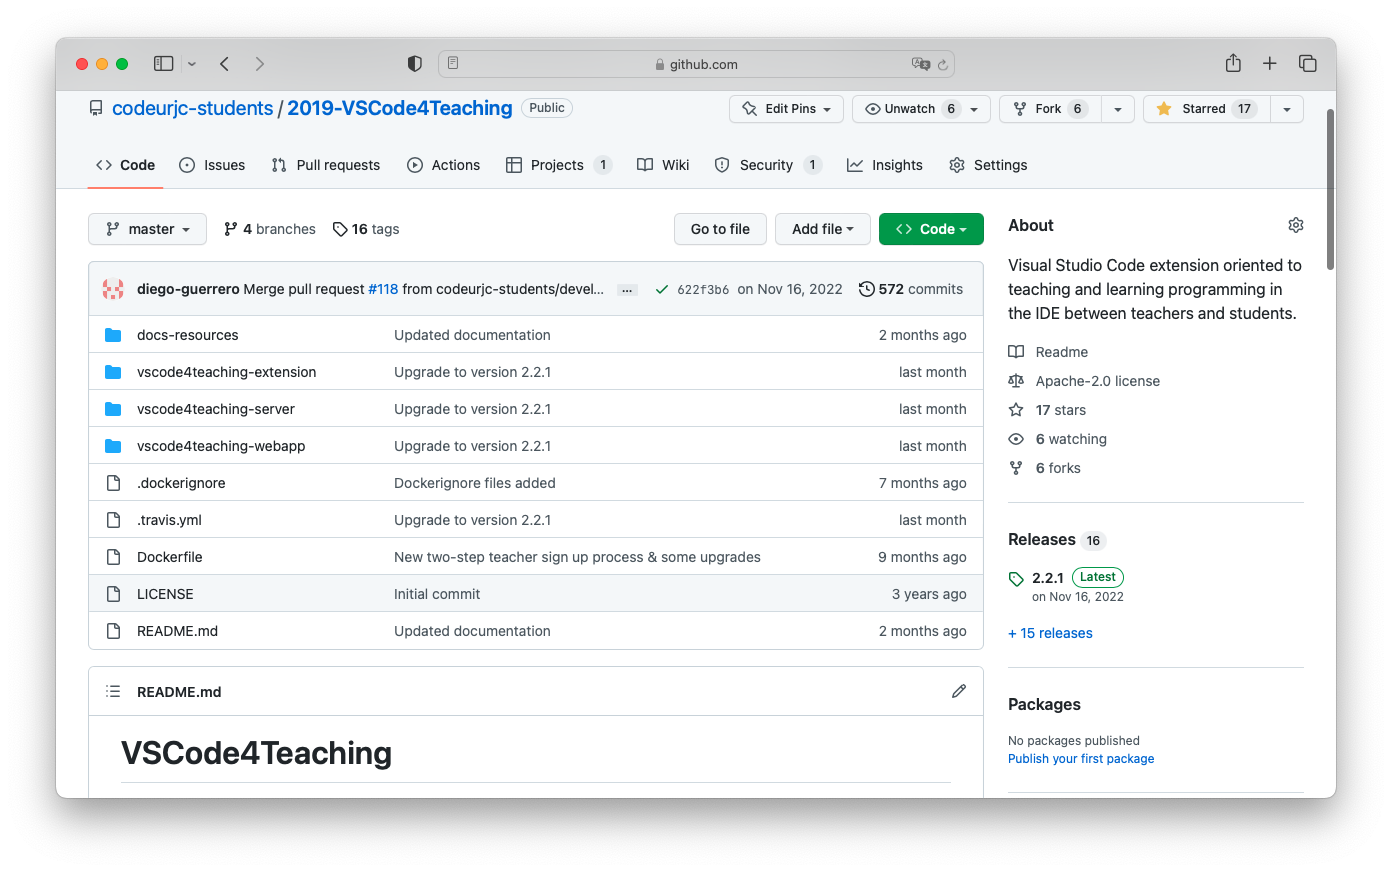
\includegraphics[width=\textwidth]{imagenes/utilizadas/4-5-distribDespliegue/repoGitHub.png}
    \caption{Repositorio de \textit{VSCode4Teaching} en GitHub.}
    \label{fig:repoGitHub}
\end{figure}

\subsection{Versiones de \textit{VSCode4Teaching} publicadas}
El proyecto \textit{VSCode4Teaching} sigue la estrategia de ``versionado semántico'' (del inglés \textit{Semantic Versioning}) \cite{Deploy_SemVer} para la designación de sus versiones. Este formato propone la nomenclatura de las versiones publicadas a través de un identificador con tres números separados por puntos; esto es, con el aspecto \texttt{X.Y.Z}. Sobre este identificador, el número \texttt{Z} aumenta en una unidad cuando la versión únicamente corrige errores menores; el número \texttt{Y}, cuando se añade funcionalidad retrocompatible; y el número \texttt{X}, cuando se introducen cambios no retrocompatibles.

El presente Trabajo Fin de Grado tomó como punto de partida la versión 2.0.2 del proyecto \textit{VSCode4Teaching}. A partir de esta versión, se han divulgado un total de siete nuevas versiones. Las versiones más destacadas publicadas y divulgadas durante el desarrollo del presente trabajo son:
\begin{itemize}
    \item Versión \textbf{2.1.4}. Fue lanzada el 29 de julio de 2022 tras tres versiones previas sobre las que se corrigieron errores. Esta versión introdujo las implementaciones de los requisitos \referenciaConTT{subsec:rf1}{RF-1}, \referenciaConTT{subsec:rf2}{RF-2}, \referenciaConTT{subsec:rf3}{RF-3}, \referenciaConTT{subsec:rf4}{RF-4}, \referenciaConTT{subsec:rf9}{RF-9}, \referenciaConTT{subsec:rf10}{RF-10} y la ejecución al menos una vez de todos los requisitos no funcionales. Se puede acceder al código de esta versión en el repositorio de GitHub a través del enlace:
    \vspace{-0.25\baselineskip}
    \begin{center}
        \href{https://github.com/codeurjc-students/2019-VSCode4Teaching/releases/tag/2.1.4}{https://github.com/codeurjc-students/2019-VSCode4Teaching/releases/tag/2.1.4}
    \end{center}
    \vspace{-0.25\baselineskip}

    \item Versión \textbf{2.2.0}. Fue lanzada el 30 de octubre de 2022, e incorporó como novedades la implementación de los requisitos \referenciaConTT{subsec:rf5}{RF-5}, \referenciaConTT{subsec:rf6}{RF-6}, \referenciaConTT{subsec:rf7}{RF-7}, \referenciaConTT{subsec:rf8}{RF-8}, \referenciaConTT{subsec:rf11}{RF-11} y \referenciaConTT{subsec:rf12}{RF-12}; y una nueva ejecución de los requisitos \referenciaConTT{subsec:rn1}{RN-1} y \referenciaConTT{subsec:rn4}{RN-4}. Análogamente, se puede visualizar en GitHub esta versión accediendo al enlace siguiente:
    \vspace{-0.5\baselineskip}
    \begin{center}
        \href{https://github.com/codeurjc-students/2019-VSCode4Teaching/releases/tag/2.2.0}{https://github.com/codeurjc-students/2019-VSCode4Teaching/releases/tag/2.2.0}
    \end{center}
    \vspace{-0.5\baselineskip}

    Esta versión se vio complementada por la \textbf{2.2.1}, lanzada el 16 de noviembre de 2022, incorporando modificaciones en las dependencias en cumplimiento del requisito \referenciaConTT{subsec:rn1}{RN-1}.
\end{itemize}

% Adicionalmente, se pueden visualizar registros de los cambios incorporados en cada versión de las anteriormente destacadas en el \textit{blog} mantenido durante el transcurso del Trabajo Fin de Grado, accesible a través del siguiente enlace:
% \vspace{-0.5\baselineskip}
% \begin{center}
%     \href{https://medium.com/@diego-guerrero}{https://medium.com/@diego-guerrero}
% \end{center}
% \vspace{-0.5\baselineskip}

\subsection{Despliegue y distribución del servidor}
Tal como se recoge en la \referenciaSeccion{subsec:tecDistribDespliegue}, Docker es una tecnología que facilita los procesos de despliegue y distribución del \textit{software}, ya que permite generar imágenes de programas multiplataforma; esto es, que pueden ser instanciadas como contenedores en cualquier computador con sistemas operativos Windows, macOS o en cualquier distribución de Linux.

El servidor y aplicación web disponen de la configuración adecuada para generar una imagen Docker que permita acceder al servidor (tal como se estipula en el requisito \texttt{RN-3}, desarrollado en la \referenciaSeccion{subsec:rn3}), introduciendo en él previamente durante el proceso de compilación la aplicación web Angular construida en forma de página construida. Esta configuración se introduce en el fichero \texttt{Dockerfile} presente en el directorio raíz.

Una de las formas más sencillas disponible para desplegar una instancia del servidor de \textit{VSCode4Teaching} es hacer uso de la configuración de \textit{Docker Compose} ---tecnología descrita en la sección anteriormente referenciada---, desarrollada e introducida dentro de la implementación del componente servidor (fichero \texttt{docker-compose.yml}).

Una de las posibilidades que Docker brinda a la comunidad de desarrolladores es la de divulgar las imágenes generadas en un repositorio en Internet, Docker Hub, que es una forma simple de ``crear, gestionar y desplegar las aplicaciones [...] en contenedores'' \cite{Deploy_DockerHub}. El servidor, construido tal como se especifica en el \texttt{Dockerfile}, se encuentra publicado en Docker Hub con el nombre \texttt{vscode4teaching/vscode4teaching}. La apariencia de la página de \textit{VSCode4Teaching} en Docker Hub se muestra en la \referenciaFigura{fig:distrib1}, y es accesible en navegadores web a través del enlace:
\vspace{-0.5\baselineskip}
\begin{center}
    \href{https://hub.docker.com/r/vscode4teaching/vscode4teaching}{https://hub.docker.com/r/vscode4teaching/vscode4teaching}.
\end{center}
\vspace{-0.5\baselineskip}

\begin{figure}[ht]
    \centering
    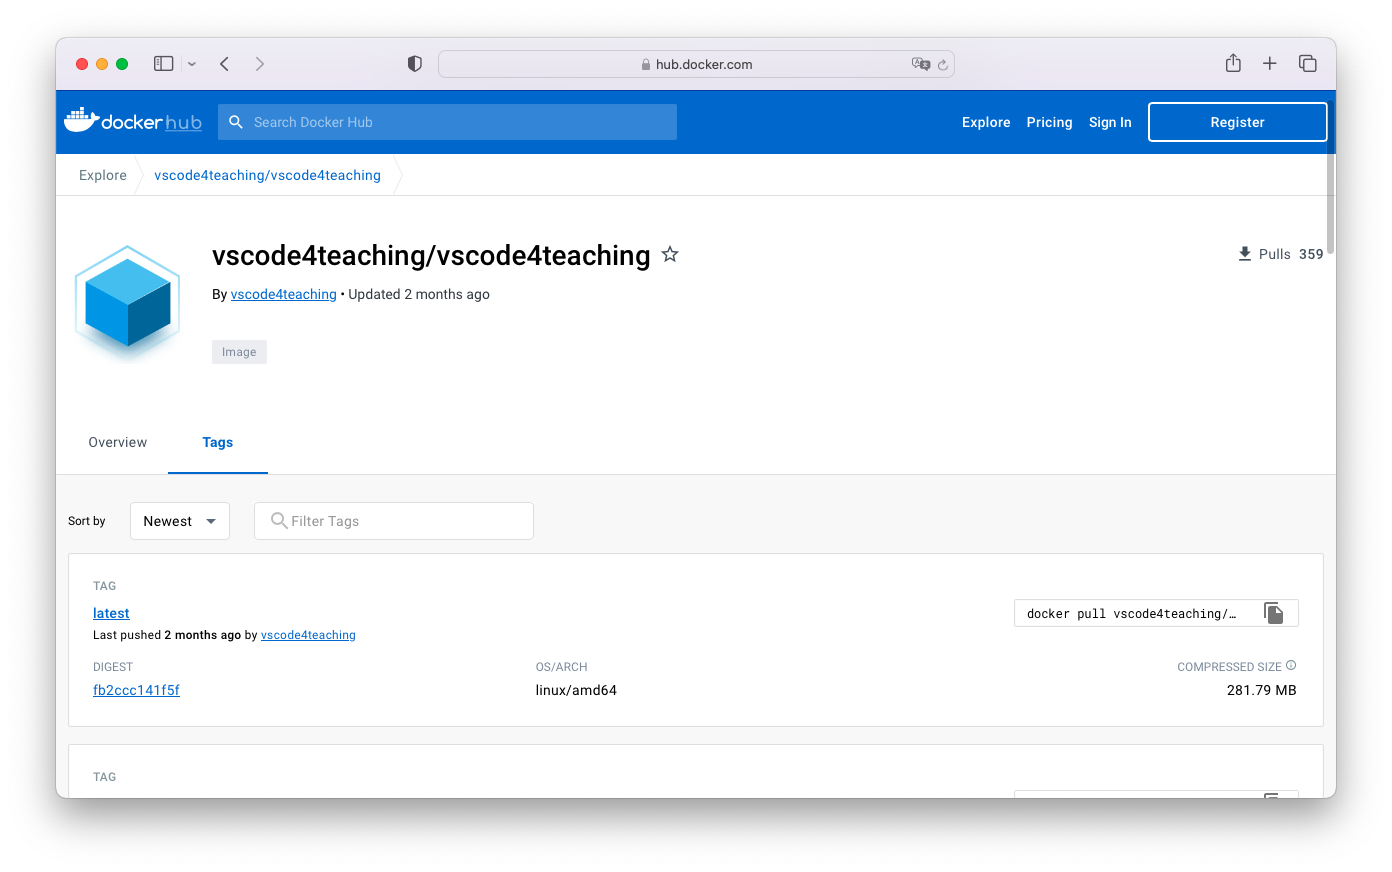
\includegraphics[width=\textwidth]{imagenes/utilizadas/4-5-distribDespliegue/capturaDockerHub.png}
    \caption{Apariencia de la página de \textit{VSCode4Teaching} en Docker Hub.}
    \label{fig:distrib1}
\end{figure}

\subsection{Distribución de la extensión}
Uno de los métodos para la divulgación de extensiones para Visual Studio Code es el \textit{Marketplace}, que es un repositorio que se pone a disposición de los desarrolladores registrados y que permite que ``otros puedan buscar, descargar y utilizar la extensión'' \cite{Tec_VSCPublish}, de modo que cualquier usuario puede descargarla directamente desde el propio entorno de desarrollo o a través de la web, tal como se puede ver en la \referenciaFigura{fig:distrib2}. La extensión ha sido publicada con el nombre \textit{VS Code 4 Teaching}, y se puede visualizar su página de información y descargar a través del enlace:
\vspace{-0.5\baselineskip}
\begin{center}
    \href{https://marketplace.visualstudio.com/items?itemName=VSCode4Teaching.vscode4teaching}{https://marketplace.visualstudio.com/items \\ ?itemName=VSCode4Teaching.vscode4teaching}.
\end{center}
\vspace{-0.5\baselineskip}


\begin{figure}[ht]
    \centering
    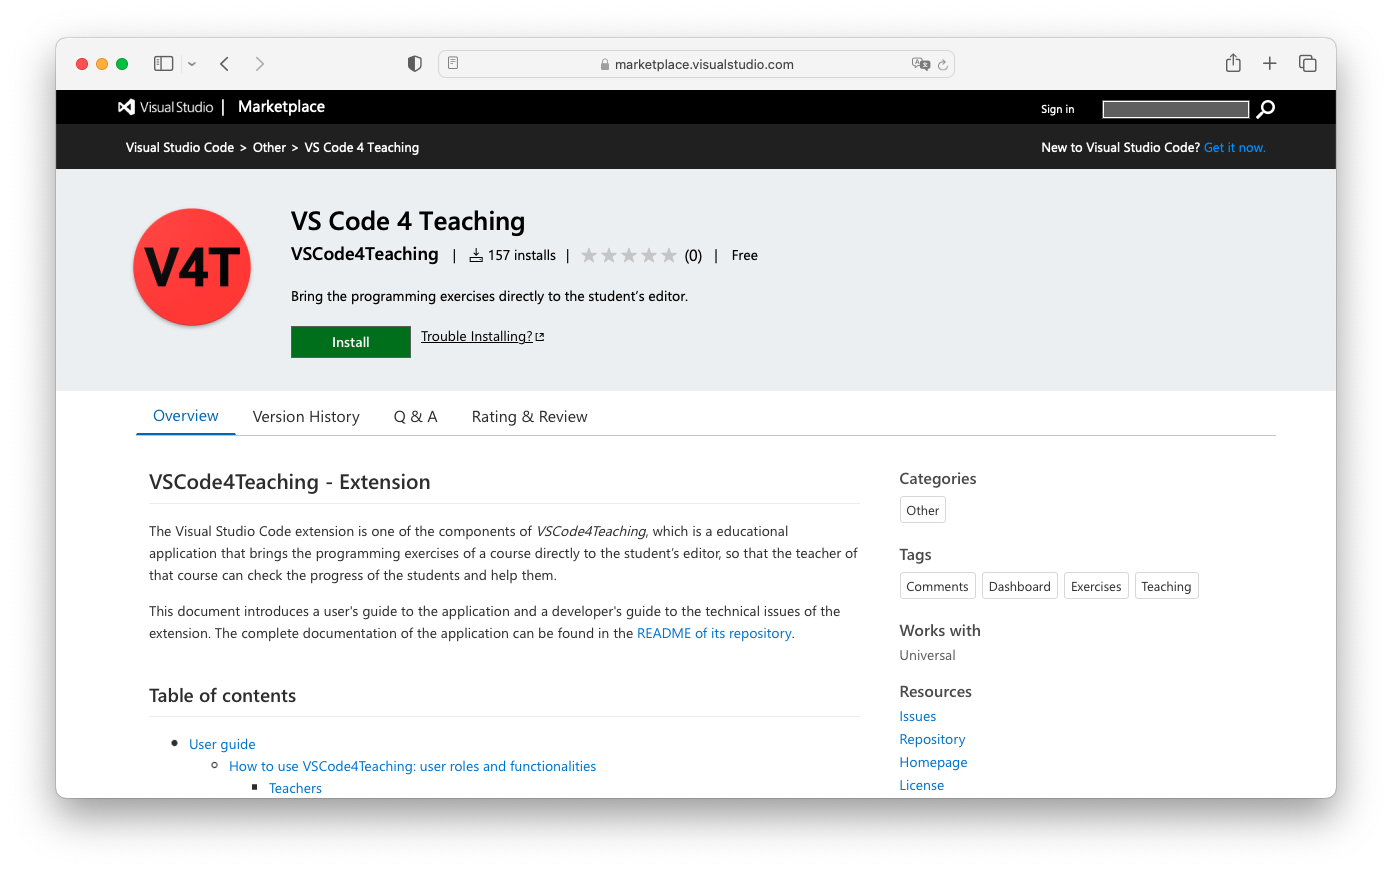
\includegraphics[width=\textwidth]{imagenes/utilizadas/4-5-distribDespliegue/capturaVSCodeMarketplace.png}
    \caption{Apariencia de \textit{VSCode4Teaching} en el \textit{Marketplace} de Visual Studio Code.}
    \label{fig:distrib2}
\end{figure}
